\chapter{Introdução}
\label{cap:introducao}
\daniel{Não falei de provedor nem cliente, pois isso só foi explicado lá no referencial teórico. Por isso aqui eu falo 'pacotes que dependem de outros'}

O \textit{Node Package Manager} (NPM) é um gerenciador de pacotes para o \textit{Node.js} e que possui um \textit{website}\footnote{https://npmjs.org}, no qual se pode consultar os pacotes, e um registro\footnote{http://registry.npmjs.org/}, no qual os pacotes publicados são hospedados. Lançado em 2009, seu principal objetivo é facilitar o compartilhamento de códigos escritos em \textit{JavaScript} -- além de outras linguagens de programação. Atualmente, o NPM ocupa a posição de maior repositório para uma dada linguagem, com mais de 1 milhão de pacotes\footnote{http://www.modulecounts.com} e continua a crescer rapidamente. O NPM é um dos que impulsionaram o \textit{JavaScript} a se tornar um ecossistema completo, com pacotes, \textit{frameworks}, aplicativos \textit{mobiles}, aplicativos \textit{web} entre outros \cite{introduction:npm} e também,  97\% dos aplicativos \textit{web} são oriundos do NPM\footnote{https://blog.npmjs.org/post/180868064080/this-year-in-javascript-2018-in-review-and-npms}

O NPM estimula o compartilhamento de código entre os pacotes e, por causa disso, contém o maior número de dependências entre os pacotes \cite{teorical_reference:npm_2}. Dessa maneira, como muitos pacotes estão dependendo mutuamente, há uma rede que interconecta os pacotes, e quando há um erro em algum dos pacotes, um grande número de pacotes, que dependem do pacote errôneo, podem ser afetados. Foi exatamente isso que ocorreu através de um pacote chamado \textit{left-pad}\footnote{https://blog.npmjs.org/post/141577284765/kik-left-pad-and-npm}. Esse pacote foi removido do NPM por seu desenvolvedor e impactou milhares de outros pacotes em apenas 2.5 horas, incluindo pacotes renomados como o \textit{babel}\footnote{https://github.com/babel/babel} e o \textit{atom}\footnote{https://github.com/atom/atom} que propagaram essa quebra de dependência para inúmeros outros pacotes. Assim, problemas de comunicação entre os pacotes realmente ocorrem no ecossistema do NPM e por isso esse foi escolhido como estudo de caso, devido à rede de interconectividade entre os pacotes.

Um defeito que causa problemas de comunicações entre os pacotes são as \textit{breaking changes}, descritas na Seção \ref{ref-teo:breaking_change}. Uma \textit{breaking change} é uma alteração em um pacote que o torna incompatível com as suas versões anteriores \cite{intro:break_change}, fazendo com que os dependentes do pacote que contém uma \textit{breaking change} tenham um comportamento indesejado. Um exemplo de \textit{breaking change} ocorreu na \textit{release optipng@0.2.0} na qual o método \textit{OptiPng.getBinaryPath} foi renomado para \textit{OptiPng.getBinPath}\footnote{https://github.com/papandreou/node-optipng/compare/v0.1.1...v0.2.0\#diff-366460cd3c3170c9c84340631e6f8e4fL22-R19}. Porém, o método foi renomeado por engano e a \textit{release} errônea foi publicada em uma versão \textit{minor} -- nível de versão do Versionamento Semântico, especificado na Seção \ref{ref-teo:semver} --, fazendo com que todos os pacotes que tinham acesso a aquele método não o tivesse mais. Assim, o código \ref{cod:bc:optipng} executa normalmente com o \textit{optipng@0.1.1}, mas ao atualizar para o \textit{optipng@0.2.0}, esse código sofre uma \textit{breaking change} -- o que não deveria acontecer com uma \textit{release minor}.

\begin{lstlisting}[style=Javascript, label=cod:bc:optipng, caption={Código que sofre \textit{breaking change} do \textit{optipng}}]
var OptiPng = require('optipng');
var cb = {apply: () => {}};
OptiPng.getBinaryPath(cb);
\end{lstlisting}

Apesar de ser um erro facilmente detectável, esse foi consertado somente após 34 dias, conforme mostra a Figura \ref{fig:bc_optipng}. Esta correção foi realizada em um \textit{commit}\footnote{https://github.com/papandreou/node-optipng/commit/a155f2b078224be18367847bbcbd3df3c379deea} no qual o desenvolvedor informou no comentário que a renomeação do método ocorreu por engano.

\begin{figure}
    \centering
    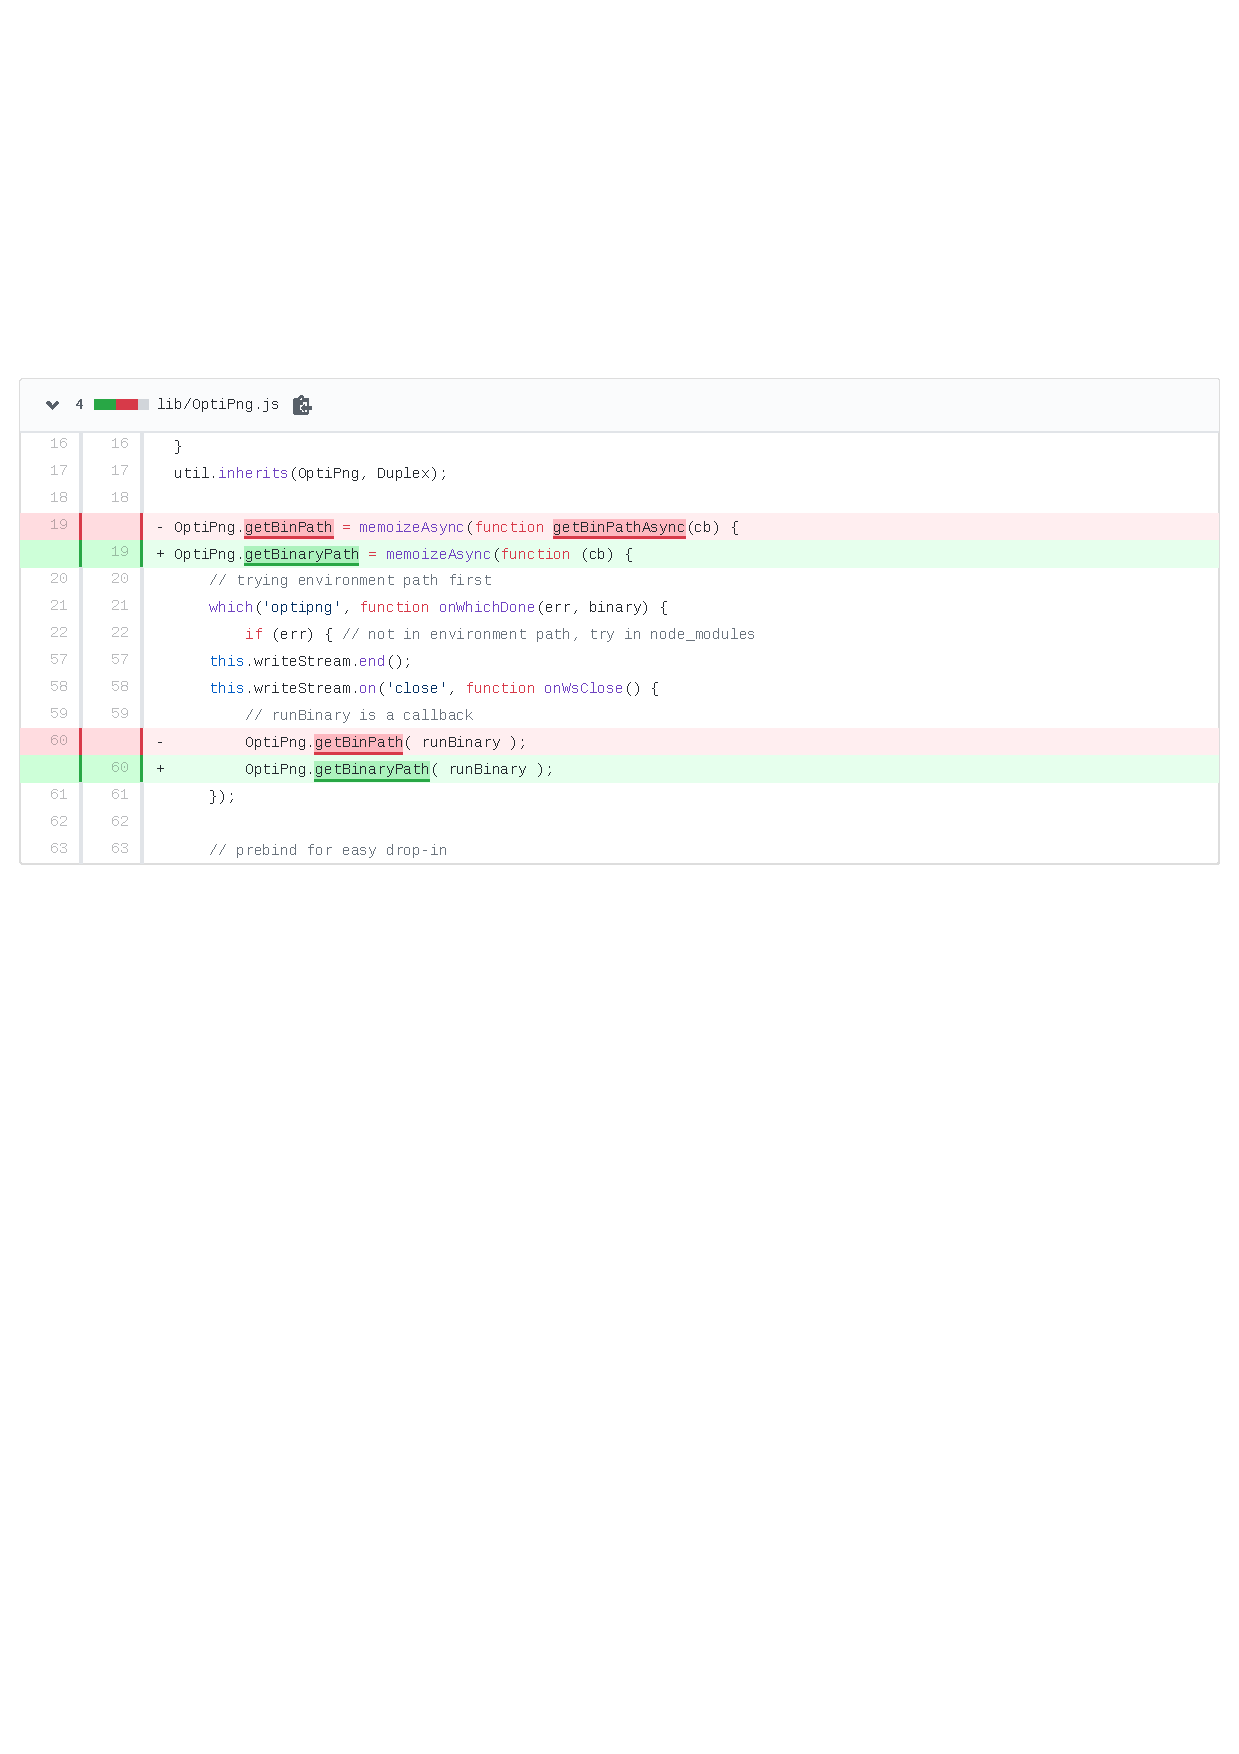
\includegraphics[scale=0.65]{figuras/bc_example.pdf}
    \caption{\textit{Commit} que corrigiu a \textit{breaking change}}
    \label{fig:bc_optipng}
\end{figure}{}

Alterações no código que causam \textit{breaking change} devem ser introduzidas em \textit{releases} versionadas com o incremento do nível \textit{major}, seguindo a especificação do Versionamento Semântico. Assim, um pacote que depende de outro pode especificar se deseja ou não receber as \textit{releases} que contêm \textit{breaking change}. Entretanto, pesquisas relacionadas mostram que as \textit{breaking changes} são introduzidas erroneamente em \textit{releases}, assim, impactando os demais pacotes. \citeonline{teorical_reference:bc_1} constatou que 9\% das \textit{releases} dos três pacotes com mais dependentes no NPM introduziram \textit{breaking changes} indevidamente e \citeonline{noregrets2018} apresentou uma ferramenta para detecção de \textit{breaking changes} e também constatou que 9\% das \textit{releases} introduziram \textit{breaking changes} quando não deveriam introduzir.

Além de quantificar as \textit{breaking changes} no ecossistema do NPM, este trabalho apresenta uma proposta para categorizar essas \textit{breaking changes} e verificar os impactos que elas causaram nos pacote. Para isso, foi utilizado uma amostra representativa dos pacotes do NPM e, para cada uma de suas \textit{releases}, foi verificado se houve alteração nas \textit{releases} aceitáveis dos pacotes que elas dependem. Então, as dependências foram resolvidas para a última versão disponível no momento da \textit{release}. Então as \textit{releases} foram executadas através dos \textit{scripts npm install/npm test}. Após, foi feita uma análise manual no código das \textit{releases} que resultaram em erro para confirmar se o erro se tratava de uma \textit{breaking change} ou não. Foi feita uma análise no repositório do pacote causador da \textit{breaking change} para recuperar informações, tais como, tipo de \textit{breaking change}, tempo que levou até ser consertada, o nível da versão que a \textit{breaking change} foi introduzida/consertada.

% isso estava nos results
%\filipe{o erro sempre se manifesta no cliente, acho que o lance é que você consegue identificar se o erro foi proveniente de uma chamada a uma função do provedor ou do próprio cliente (ou algum outro provedor que não interessa à análise).}

%\filipe{breaking change (defeito no provedor) vs. manifestação da breaking change (manifestação do defeito do provedor no cliente)}